\documentclass{standalone}
\usepackage{tikz}
\usetikzlibrary{chains}
\begin{document}
	
	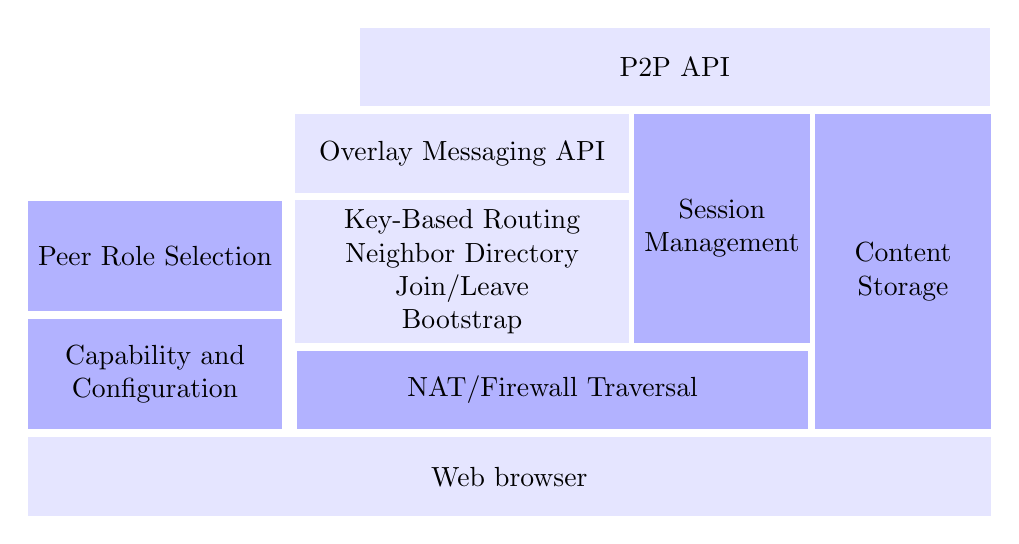
\begin{tikzpicture}[
	node distance=11mm,
	minimum height=10mm,
	text centered,
	desc/.style={
		rectangle,
		fill=blue!30
	},
	sm/.style={
	text width=3cm,
	minimum height=14mm,
	node distance=15mm, xshift=-45mm
	},
	me/.style={
	text width=4cm, xshift=-6mm
	},
	it/.style={
		fill=blue!10
	},
	lg/.style={
	text width=20mm,
	minimum height=40mm,
	yshift=15mm
	}
	]
	
	

	\node [desc,it,text width=12cm] (App) {Web browser};
	\node [desc,me, above of=App,text width=62.5mm, xshift=11.5mm] (NAT) {NAT/Firewall Traversal};
	\node [desc,me, it, above of=App, yshift=15mm] (Core) {Key-Based Routing\\ Neighbor Directory\\ Join/Leave \\Bootstrap};
	
	\node [desc, sm,above of=App,yshift=-2mm	] (Capability) {Capability and Configuration};	
	\node [desc, sm,above of=App,yshift=13mm] (Role) {Peer Role Selection};
	
	\node [desc,lg,above of=App, xshift=50mm] (Content) {Content Storage};
	\node [desc,above of=App, 
	minimum height=29mm,
	text width=20mm,
	yshift=20.5mm,xshift=27mm] (Session) {Session \\Management};
	
	\node [desc,me, it, above of=App, yshift=30mm] (Overlay) {Overlay Messaging API};
	
	\node [desc,me, it, above of=Overlay, xshift=33mm,minimum width=8cm] (P2P) {P2P API};
	
	\end{tikzpicture}
	\end{document}